\documentclass{article}
\usepackage[a4paper, margin=2cm]{geometry}
\usepackage{tikz}
\usetikzlibrary{arrows.meta, bending}
\usepackage{xcolor}

% Inline event-mention box — identical to the reference template
\newcommand{\tikzmarkbox}[3][]{%
  \tikz[remember picture, baseline=(#2.base)]%
    \node[
      draw=blue,
      fill=blue!10,
      rectangle,
      rounded corners,
      inner sep=1pt,
      outer sep=0pt,
      #1,
      anchor=base
    ] (#2) {#3};%
}

\parindent=0pt
\begin{document}

\begin{figure}[htbp]
\centering

{\normalsize\bfseries EventStoryLine~0.9\enspace$\cdot$\enspace\texttt{1\_7ecbplus.xml}}

\medskip

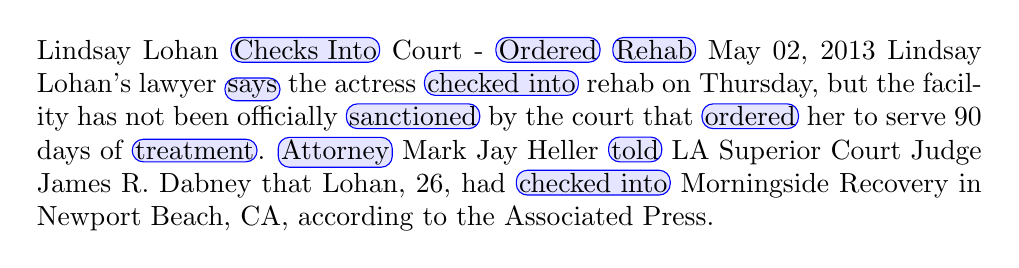
\begin{tikzpicture}[remember picture]
\node[text width=12.0cm, align=justify] (mainText) {%
Lindsay Lohan \tikzmarkbox{n1}{Checks Into} Court - \tikzmarkbox{n7}{Ordered} \tikzmarkbox{n27}{Rehab} May 02, 2013 Lindsay Lohan's lawyer \tikzmarkbox{n9}{says} the actress \tikzmarkbox{n2}{checked into} rehab on Thursday, but the facility has not been officially \tikzmarkbox{n3}{sanctioned} by the court that \tikzmarkbox{n4}{ordered} her to serve 90 days of \tikzmarkbox{n5}{treatment}. \tikzmarkbox{n10}{Attorney} Mark Jay Heller \tikzmarkbox{n8}{told} LA Superior Court Judge James R. Dabney that Lohan, 26, had \tikzmarkbox{n6}{checked into} Morningside Recovery in Newport Beach, CA, according to the Associated Press.%
};
\end{tikzpicture}

\medskip

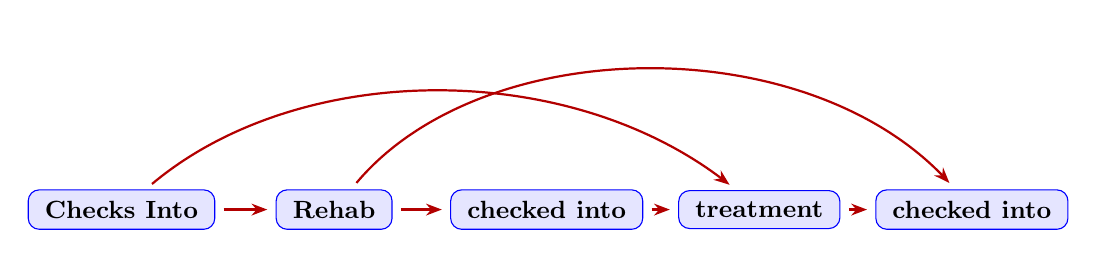
\begin{tikzpicture}[
  event/.style={draw=blue, fill=blue!10, rounded corners,
    inner xsep=6pt, inner ysep=4pt, font=\small\bfseries},
  causes/.style={-{Stealth[length=2mm]}, thick, red!70!black, shorten <=3pt, shorten >=3pt}
]
  \node[event] (n1) at (0.6, 0.0) {Checks Into};
  \node[event] (n2) at (6.0, 0.0) {checked into};
  \node[event] (n5) at (8.7, 0.0) {treatment};
  \node[event] (n6) at (11.4, 0.0) {checked into};
  \node[event] (n27) at (3.3, 0.0) {Rehab};

  \draw[causes] (n27) -- (n2);
  \draw[causes] (n27) to[out=50, in=130, looseness=0.89] (n6);
  \draw[causes] (n2) -- (n5);
  \draw[causes] (n1) -- (n27);
  \draw[causes] (n5) -- (n6);
  \draw[causes] (n1) to[out=40, in=140, looseness=0.89] (n5);
\end{tikzpicture}

\smallskip

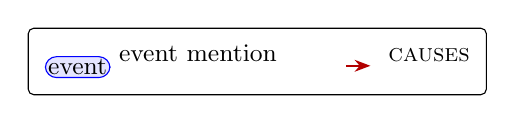
\begin{tikzpicture}
\node[draw, fill=white, font=\small, anchor=north,
      inner sep=6pt, rounded corners=2pt] {%
  \tikz[baseline=-0.5ex]{\node[draw=blue, fill=blue!10,
    rounded corners, inner sep=1pt, font=\small]{event};} event mention
  \qquad
  \tikz[baseline=0.4ex]{\draw[-{Stealth[length=2mm]}, thick, red!70!black, shorten <=3pt, shorten >=3pt](0,0)--(1.6em,0);}  \textsc{causes}%
};
\end{tikzpicture}

\caption{Annotated example from EventStoryLine~0.9 (\texttt{1\_7ecbplus.xml}). Blue boxes are event mentions. Arrows show \textsc{causes} relations.}
\label{fig:1-7ecbplus-xml}
\end{figure}

\end{document}
